\documentclass[runningheads]{llncs}

% ---------------------------------------------------------------
% Include basic ECCV package
 
% TODO REVIEW: Insert your submission number below by replacing '*****'
% TODO FINAL: Comment out the following line for the camera-ready version
\usepackage[review,year=2026,ID=*****]{eccv}
% TODO FINAL: Un-comment the following line for the camera-ready version
%\usepackage{eccv}

% OPTIONAL: Un-comment the following line for a version which is easier to read
% on small portrait-orientation screens (e.g., mobile phones, or beside other windows)
%\usepackage[mobile]{eccv}


% ---------------------------------------------------------------
% Other packages

% Commonly used abbreviations (\eg, \ie, \etc, \cf, \etal, etc.)
\usepackage{eccvabbrv}

% Include other packages here, before hyperref.
\usepackage{graphicx}
\usepackage{booktabs}

% The "axessiblity" package can be found at: https://ctan.org/pkg/axessibility?lang=en
\usepackage[accsupp]{axessibility}  % Improves PDF readability for those with disabilities.


% ---------------------------------------------------------------
% Hyperref package

% It is strongly recommended to use hyperref, especially for the review version.
% Please disable hyperref *only* if you encounter grave issues.
% hyperref with option pagebackref eases the reviewers' job, but should be disabled for the final version.
%
% If you comment hyperref and then uncomment it, you should delete
% main.aux before re-running LaTeX.
% (Or just hit 'q' on the first LaTeX run, let it finish, and you
%  should be clear).

% TODO FINAL: Comment out the following line for the camera-ready version
%\usepackage[pagebackref,breaklinks,colorlinks,citecolor=eccvblue]{hyperref}
% TODO FINAL: Un-comment the following line for the camera-ready version
\usepackage{hyperref}

% Support for ORCID icon
\usepackage{orcidlink}



%%%%%%%%% TITLE - PLEASE UPDATE
\title{\ourmethod{}: Intersection-Free Mesh to Mesh Composition}

%%
%% authors

%%
%% abstract

%%%%%%%%% AUTHORS - PLEASE UPDATE
\author{First Author\\
Institution1\\
Institution1 address\\
{\tt\small firstauthor@i1.org}
% For a paper whose authors are all at the same institution,
% omit the following lines up until the closing ``}''.
% Additional authors and addresses can be added with ``\and'',


\begin{document}


\maketitle
\begin{center}
    \centering
    %\vspace{-2cm}
    
\includegraphics[width=\linewidth]{figures/teaser/teaser.pdf}
    \captionof{figure}{\ourmethod{} is a multi-step optimization algorithm that fits accessories onto meshes realistically, tightly, and without intersections.}
    % and even deforming the accessory if its material allows.}
    % \captionof{figure}{\ourmethod{} is capable of fitting various mesh objects onto user-defined target regions defined over a base mesh (the Max Planck mesh). Our method finds a semantically and physically realistic fit by rigidly permuting and non-rigidly deforming the fitted objects, while strictly preventing any surface intersections. The figure shows how our method can be applied iteratively to create a composition of various wearables. Notice how each object is fitted respective of their supposed materials--the face mask deforms and fits elastically over the contours of the lower face, the eye mask slightly less so, while the helmet remains completely rigid.}
    %\vspace{-2cm}
    \label{fig:teaser}
\end{center}%


% \maketitle

%%
%% The abstract is a short summary of the work to be presented in the
%% article.
\begin{abstract}
We propose \ourmethod{}, a method that finds physically and semantically realistic compositions of two input meshes. Given an accessory, a base mesh with a user-defined target region, and optional text strings for both meshes, \ourmethod{} uses a multi-step optimization framework to realistically fit the meshes onto each other while preventing intersections.
We initialize the shapes' rigid configuration via a structured alignment scheme using Vision-to-Language Models, which we then optimize using a combination of attractive geometric losses, and a physics-inspired barrier loss that prevents surface intersections. 
We then obtain a final deformation of the object, assisted by a diffusion prior.
% To achieve a tight and non-intersecting fit, we present a novel 4-step divide-and-conquer approach, where we first tightly fit, solve for intersections, re-tighten the fit, then non-rigidly deform the accessory using both semantic and physical guidance. Usefully, our model incorporates a VLM-initialization module that uses user-input text to deduce the materials of the accessory, then tunes the materials elasticity parameters to control the degrees of deformation. 
Our method successfully fits accessories of various materials over a breadth of target regions, and is designed to fit directly into existing digital artist workflows. We demonstrate the robustness and accuracy of our pipeline by comparing it with generative approaches and traditional registration algorithms.
\end{abstract}

\section{Introduction} \label{sec:introduction}

% Narrow in
\emph{Mesh composition} is the process of assembling several pre-modeled 3D objects into a unified asset.
It is a fundamental part of many 3D content creation workflows, in which an artist selects \emph{accessories} from an existing library and manually rotates, translates and deforms them to fit realistically on a character's \emph{base mesh} without intersections (see \autoref{fig:teaser}).
Automating this tedious task is a critical and challenging research question combining \emph{geometric} and \emph{physical} constraints (the two meshes must be close to each other without intersecting) with \emph{semantic} alignment (e.g., a pair of glasses should sit on the eyes in the correct orientation).



\begin{figure*}
    \centering
    \vspace{3mm}
    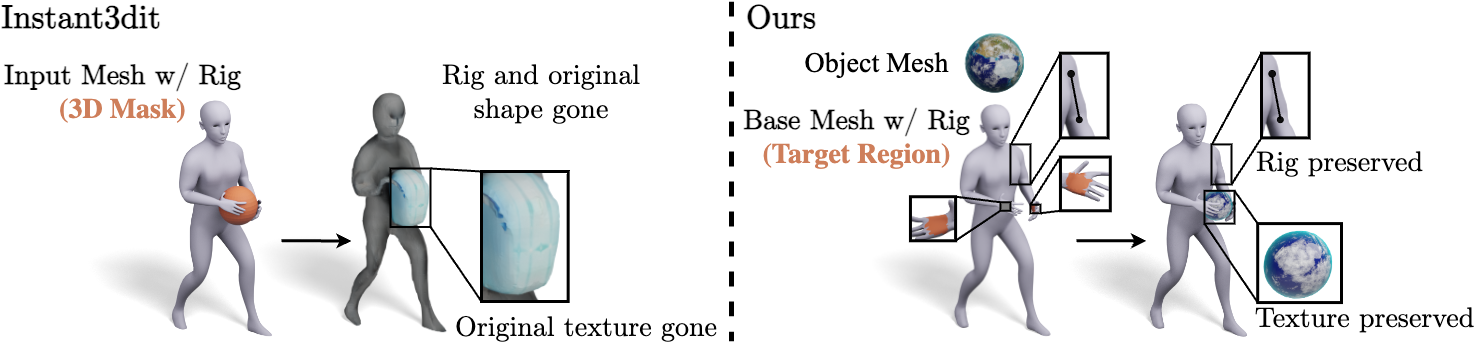
\includegraphics[width=\textwidth]{figures/instant3dit_comparison/instant3dit_comparison.png}
    \captionof{figure}{Digital artists often load shapes from pre-existing libraries of meshes that include additional information like animation rigs, skinning weights, texture maps and more. Generative shape editing methods like Instant3dit \cite{barda2025instant3dit} discard this information, performing global changes to the shapes and merging them together. \ourmethod{} is designed to fit exactly within this common artistic pipeline, and perfectly preserves all pre-existing information on the input meshes.}
    \label{fig:instant3dit_comparison}
    \vspace{-5.9mm}
\end{figure*}%


% Unfortunately, ...
However, recent advances in 3D content creation have focused mostly on \emph{generative} tasks; for example, creating shapes from text inputs~\cite{lin2023magic3d}.
These methods produce doubtlessly impressive results; yet, they do so at the cost of artist control and by relying on implicit geometric representations (e.g., radiance fields~\cite{mildenhall2021nerf} or Gaussian splats~\cite{kerbl20233d}) that are not directly usable in graphics pipelines.
Even when triangle meshes are generated~\cite{hao2024meshtron}, these are significantly lower in quality than those already available to artists in pre-existing shape libraries, lacking critical attributes like textures, animation rigs, and distinct material parameters. 







% We propose...
We propose \ourmethod{}, an optimization framework that progressively rotates, translates and then deforms an accessory until it fits tightly onto a base mesh while maximizing geometric, physical and semantic alignment.
We model this task's complexity by combining geometric losses based on distance between the meshes with physical losses preventing intersections and diffusion-based semantic guidance, and
devise a unique, multi-step optimization strategy in which each individual loss is introduced sequentially.

To succesfully navigate the ambiguities of the composition problem, we first assume that some coarse segmentation of the local ``fit'' region is highlighted, and use Vision-to-Language Model~\cite{gemini} agents to ensure adequate initialization. 
From this semantically-guided initial configuration, our algorithm drives the accessory closer to the base mesh, while using a GPU-optimized Bounding Volume Hierarchy to efficiently enforce non-intersection.
Similarly to how an artist may refine a pre-modeled accessory after optimizing its coarse position, our method optimizes a final deformation of the object through its Jacobians~\cite{aigerman2022neural}, maintaining physical realism by accounting for its (given or inferred) material parameters.










In this paper, we present a geometric optimization framework for reliably composing 3D meshes with accessories.
Through qualitative and quantitative comparisons, we show that our geometric optimization outperforms more general generative and 3D registration approaches for the task of mesh composition, while remaining intersection-free.
We show the robustness and applicability of our method on a diverse set of base meshes and accessories inspired by 3D content generation pipelines.



\begin{figure*}[t]
    \centering
    % \vspace{-0.7cm}
    \vspace{3mm}
    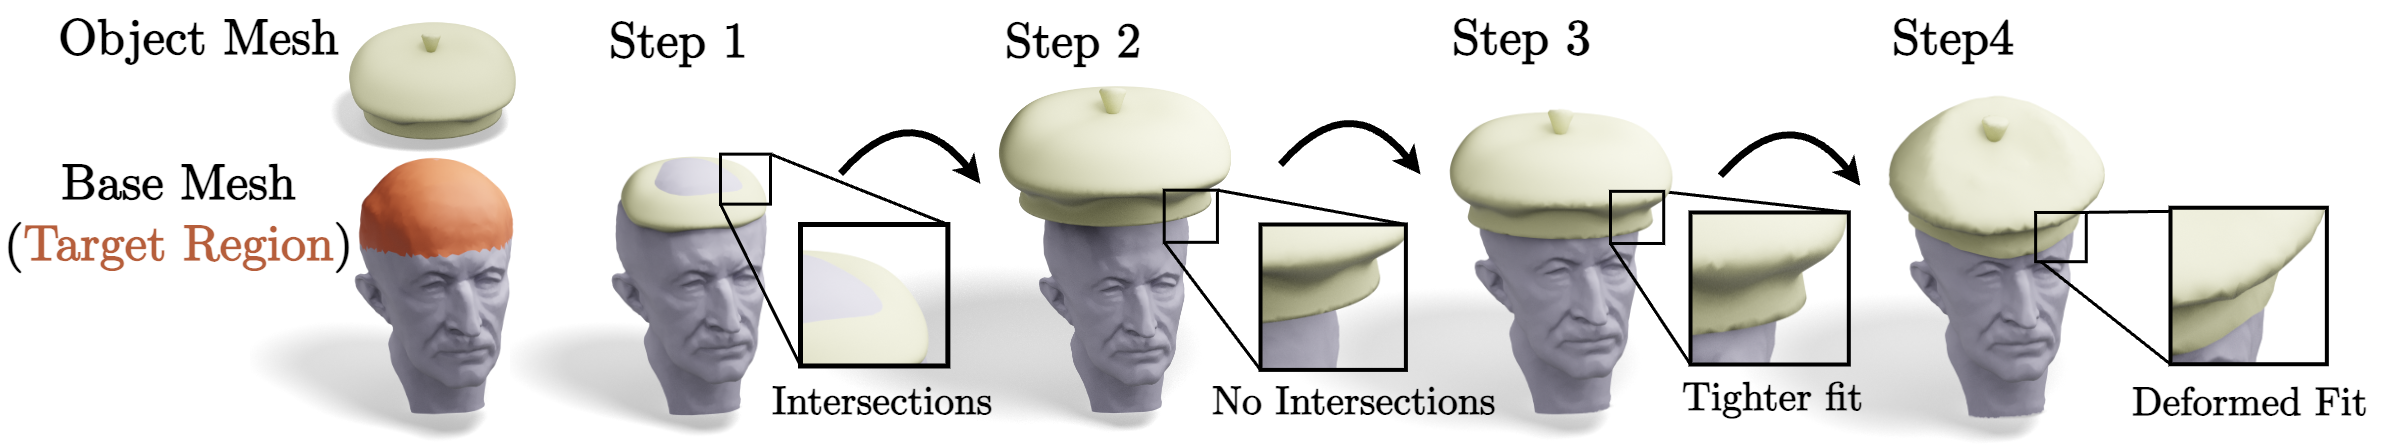
\includegraphics[width=\textwidth]{figures/main_method/main_method.png}   
    \caption{We compose the two meshes through a multi-step optimization pipeline: from an initialization obtained with a Vision-to-Language Model (\autoref{sec:initialization}), we start by obtaining a tight fit containing intersections (\autoref{sec:step1}), which we then resolve (\autoref{sec:step2}). After finetuning the fit to obtain the best possible rigid fit (\autoref{sec:step3}), we improve it further by allowing small deformations in the accessory object (\autoref{sec:step4}).}
    \label{fig:main_method}
    %\vspace{-2cm}
    \vspace{-3mm}
\end{figure*}

% \vspace{-6mm}
\section{Related Work} 

\label{sec:related_work}


\subsection{3D Registration}

The alignment of 3D objects is a fundamental problem in computer vision and graphics that has been studied thoroughly for decades \cite{mckay2003review,salvi2007survey, tam2013registration}. In this task, one seeks to find a transformation of an object to minimize an error metric defined with respect to another. A prominent work in this field is the Iterative Closest Point \cite{besl1992method,segal2009generalized}, which finds the optimal rotation and translation between two point clouds to minimize the distance between them. Among follow-up works to ICP are the globally optimal ICP (Go-ICP) \cite{yang2015go} and Fast Global Registration (FGR) \cite{zhou2016fast}.

In the deep learning era, numerous works have leveraged the power of neural networks for the registration problem, where the Euclidean distance between points has been replaced with the similarity of points in a learned feature space \cite{litany2017deep,aoki2019pointnetlk,wang2019dcp,huang2020fmr,choy2020dgr,lang2021dpc,yew2022regtr,jiang2023se}. Our mesh composition problem can be thought of as a registration problem between the asset mesh and the corresponding region on the body mesh. However, different from previous work that aligned two observations of the \textit{same} object, the asset is completely different from the target body region, making the problem highly challenging.

\subsection{Mesh Deformation}
A large body of research has been dedicated to surface deformation. Classical methods typically define an energy function subject to which the mesh is optimized, where the objective embodies desired properties of the deformed result \cite{yu2004poisson,botschsorkine08deformsurvey,skinningcourse:2014,Fulton:LSD:2018}. As-Rigid-As-Possible \cite{sorkine2007rigid} and Laplacian surface editing \cite{sorkine2004laplacian} are seminal works in this domain, which encourage smooth and rigid deformations. Such methods are applied to the subject mesh independently, without considering its interaction with other objects. 

% \itai{@someone, back me up on this independent claim, or refine as needed.}

In light of the unprecedented success of deep learning, researchers have incorporated deep foundation models as implicit guidance for the deformation process instead of the traditional hand-crafted optimization objective, leveraging the rich semantic priors embodied in these models and enjoying their intuitive language-based interface \cite{michel2022text2mesh,xu2024fusiondeformer,yang2024dreammesh,chen2024textmeshrefine}. TextDeformer \cite{michel2022text2mesh} used the CLIP model for deforming a source mesh toward a textual description, like turning a hand into an octopus. Follow-up works employed a powerful diffusion model for other deformation-driven creative applications, including concept blending \cite{kim2025meshup} and identity-preserving geometric stylization~ \cite{dinh2025geometry}. 

Similarly, we also leverage a diffusion model to guide the deformation of the accessory mesh. In contrast to prior work, the deformation in our case is constrained by the body mesh it should be composed onto, considering both their global semantic alignment and their local geometric fitting.

A recent work tackled the problem of designing creative 3D objects that fit a body mesh \cite{guo2025craft}. However, in stark contrast to our work, in CRAFT \cite{guo2025craft}, the contact points between the meshes are \textit{given} as input, while our method \textit{finds} the alignment between the meshes from a \textit{random initialization} of the asset object. 
%Additionally, the penetration avoidance between the asset and body is posed as a \textit{soft constraint}, while we \textit{guarantee} intersection-free composition of the meshes \textit{by construction}.

More relevant to our work is Instan3dit \cite{barda2025instant3dit}. In this work, the authors augment a base mesh with an accessory, such as adding a honey pot between the hands of a bear. The edit is implemented as a multi-view inpainting problem, followed by a 3D reconstruction from the posed images. While the results are visually appealing, the contact between the local edit and the body mesh is not modeled explicitly, leading to the gluing of the two. In our work, on the other hand, we consider the mesh interaction explicitly and successfully preserve the base and asset mesh properties (see \cref{fig:instant3dit_comparison}).

%\itai{I have a personal beef with this work. You might have to tone me down in this paragraph ha ha.}

%Additionally, the contact points and penetration avoidance between the asset and body are posed as \textit{soft constraints}


% \clearpage


\section{Method} 
\label{sec:method}
\vspace{-2mm}
The inputs to our method are a base mesh $\basemesh = (\baseverts, \basefaces)$ (e.g., a bust, as shown in \autoref{fig:main_method}) and an object or accessory mesh $\objectmesh = (\objectverts, \objectfaces)$ (e.g., a hat) in arbitrary relative position, together with a highlighted region of the base mesh $\highlightedmesh \subseteq \basemesh$ (the orange region in \autoref{fig:main_method}) and an optional text string describing both shapes.
The algorithm we will detail in this section will output a transformed object mesh $\transformation (\objectmesh) = (\transformation (\objectverts), \objectfaces)$ that can be superimposed with the base mesh \emph{tightly}, in a \emph{semantically and physically realistic} way \emph{without intersections}.

\begin{figure*}[t]
    \centering
    \vspace{3mm}
    %\vspace{-2cm}
    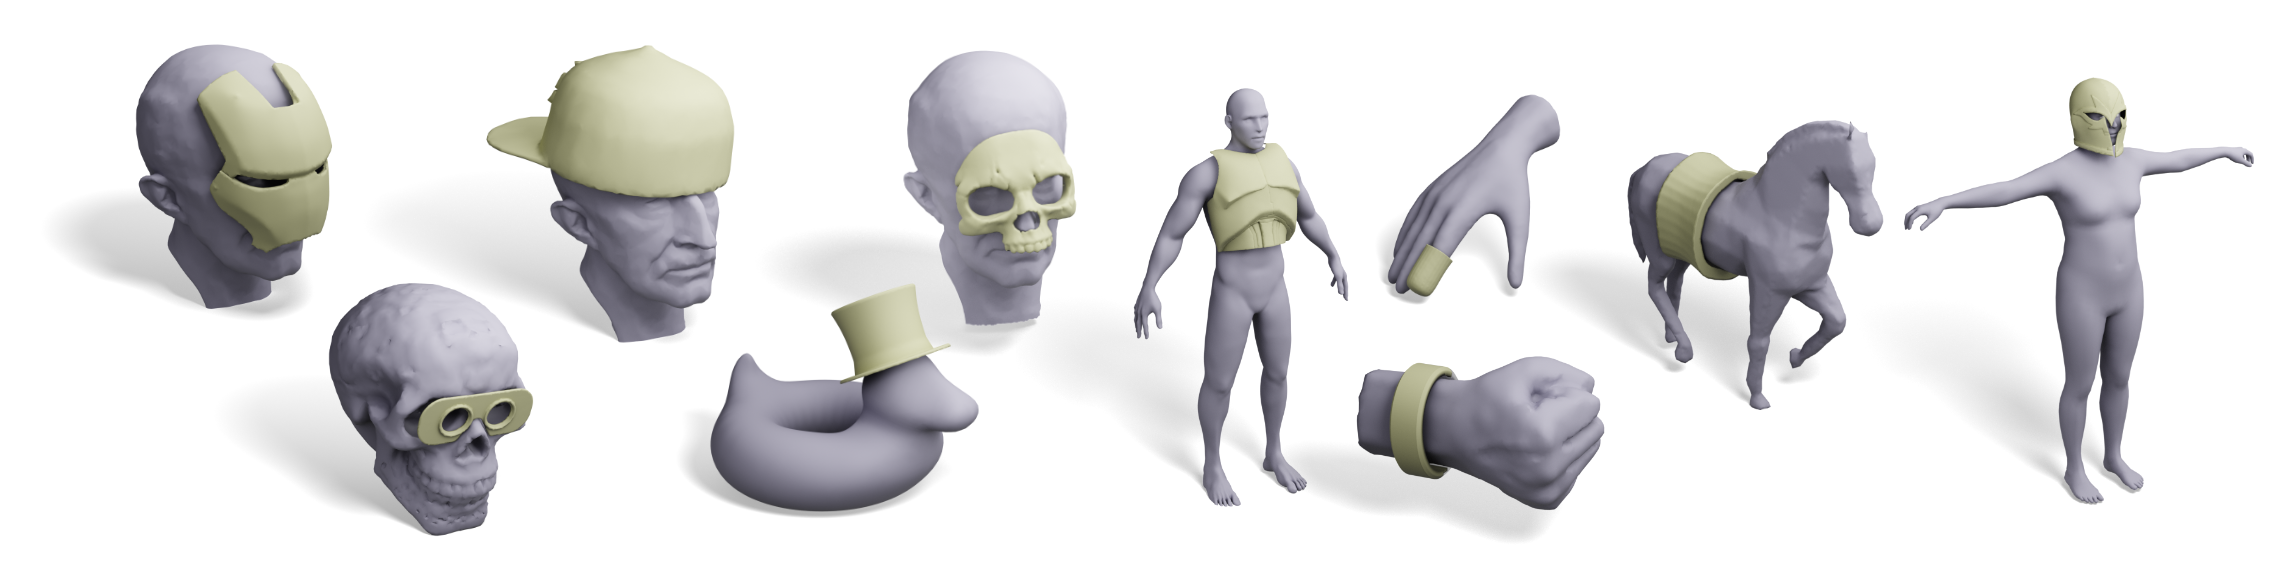
\includegraphics[width=\textwidth]{figures/gallery/gallery.png}
    \captionof{figure}{\ourmethod{} is capable of fitting a wide variety of accessories on a range of different meshes. Our method handles challenging spatial relationships such as sliding glasses along a head to align with the ears, positioning hats and helmets to conform to head curvature, wrapping bands around articulated limbs, and fitting objects along long, curved surfaces. These examples demonstrate the flexibility of our fitting trajectory and its ability to adapt accessories to widely varying shapes and poses.}
    %\vspace{-2cm}
    \label{fig:gallery}
    \vspace{-3mm}
\end{figure*}%


These goals often act in opposition to one another; for example, achieving a tighter fit will often produce intersections, while removing intersections will tend to produce a looser fit.
We address this challenge through a multi-step optimization framework in which the different constraints, objectives and degrees of freedom of the problem are introduced one at a time.
From an initial (scaled) rigid transformation $\rigid_0$ (we defer discussion of initialization strategies to \autoref{sec:initialization}), we begin by rigidly and tightly fitting the object onto the base mesh, potentially \emph{with} intersections (see $\rigid_1$ in \autoref{sec:step1}).
Then, we simulate possible rigid object attachment trajectories using physically-inspired losses to obtain a loose \emph{non-intersecting} configuration $\rigid_2$ (see \autoref{sec:step2}), which we then refine, first into a tight rigid non-intersecting fit $\rigid_3$ (see \autoref{sec:step3}) and then through a diffusion-guided deformation (see \autoref{sec:step4}) to produce our final transformation $\transformation$.


\subsection{Step 1: Tight fit with intersections}
\label{sec:step1}



We will represent the space of all possible scaled rigid transformations through rotation, translation and scale parameters $\rigid(\parameters) = \rigid (\rotation, \translation, \scale)$, where $\rotation$ are the standard continuous 6D representation of 3D rotations \cite{zhou2019continuity}.
To find a rigid transformation that aligns the object mesh with the highlighted region of the base mesh (potentially while intersecting with it), one could naively optimize the two-sided vertex-to-mesh total distance between the base and (highlighted) object meshes
\begin{equation*}
    \sum_{\vertex_{i} \in \objectmesh} d (\rigid(\parameters)\vertex_i, \highlightedmesh)^2 +  \sum_{\vertex_{j} \in \highlightedmesh} d(\vertex_j, \rigid (\parameters)\objectmesh)^2\, .
\end{equation*}
Optimizing such energy directly would present two key challenges. First, the quadratic computational complexity would place a severe limit on mesh size. Secondly, the dense computational graph would present storage and performance issues during GPU autodifferentiation.



We fix the first of these problems through a Bounding Volume Hierarchy tailor-made to exploit vectorized operations in the GPU.
We build our BVH in a similar way to a traditional Axis-Aligned Bounding Box hierarchy (see \cite{shirley2009fundamentals}, Chap. 12). However, we abort any top-down traversal when a box contains fewer than $K$ mesh triangles, resorting instead to a tensorized batch query in the GPU (in our experiments, we fix $K=1,000$).

To avoid overhead from dense computational graphs, and to make our algorithm robust to haphazardly defined contact regions, we introduce a \emph{masked} distance function $\hat{d}$ that is identical to the true distance $d$ but which zeroes out any entry above a threshold $\thresholdprox$ (in our experiments, $\thresholdprox=0.5$). This lets us define our \emph{proximity loss}
\begin{equation*}
    \mathcal{L}_{p}(\parameters) = \sum_{\vertex_{i} \in \objectmesh} \hat{d} (\rigid(\parameters)\vertex_i, \highlightedmesh)^2 +  \sum_{\vertex_{j} \in \highlightedmesh} \hat{d}(\vertex_j, \rigid (\parameters)\objectmesh)^2\, ,
\end{equation*}
which we optimize to find $\parameters^\star$ and, with it, our first scaled rigid transformation $\rigid_1 = \rigid (\parameters^\star)$ (see \autoref{fig:main_method}).




\subsection{Step 2: Trajectory-based intersection solve}
\label{sec:step2}

In the previous step, we rigidly transformed the object to tightly fit into the base mesh; however, this often introduces intersections between them (see \autoref{fig:trajectory_method}). We will now turn this intersecting configuration into a non-intersecting one, without compromising too much on tightness.


To do so, we will draw inspiration from how one puts on an accessory: for most tightly-fitting ones, there exists a valid, intersection-free trajectory that moves the object from a detached configuration into a tight fit with the base mesh (e.g., the process of putting on a hat or a ring).

We will begin by generating a large number of potential starting points for this trajectory, as shown in \autoref{fig:trajectory_method}. To do so, we draw rigid transformation's parameters from independent Gaussian and uniform distributions
\begin{align*}
\mathbf{e}_i \sim \gaussian (0,\sigma_{rot})\,,&\quad \scale \sim \uniform(\scale_{\min}, \scale_{\max})\,,\\
\translation_{\perp} \sim \gaussian (0,\sigma_{\perp})\,,&\quad \translation_{\parallel} \sim \gaussian (\mu_{\parallel},\sigma_{\parallel})
\end{align*}
where we have separated $\translation$ into the components orthogonal ($\translation_{\perp}$) and parallel ($\translation_{\parallel}$) to the average normal in the base mesh's highlighted region $\highlightednormal$ (see \autoref{fig:trajectory_method}, left). We draw samples from these distributions to produce candidate scaled rigid transformations $\rigid$ and check whether $\rigid \objectmesh$ intersects with the base mesh $\basemesh$, repeating this sampling process and progressively increasing the values of $\sigma_{rot}$ and $\sigma_{\parallel}$ until we find $\numnonintersecting$ non-intersecting candidate transforms $\rigid^1,\dots,\rigid^{\numnonintersecting}$ (in our experiments, $\numnonintersecting = 100$).

\begin{wrapfigure}[9]{r}{0.55\linewidth}
    \centering
    \vspace{-6mm}
    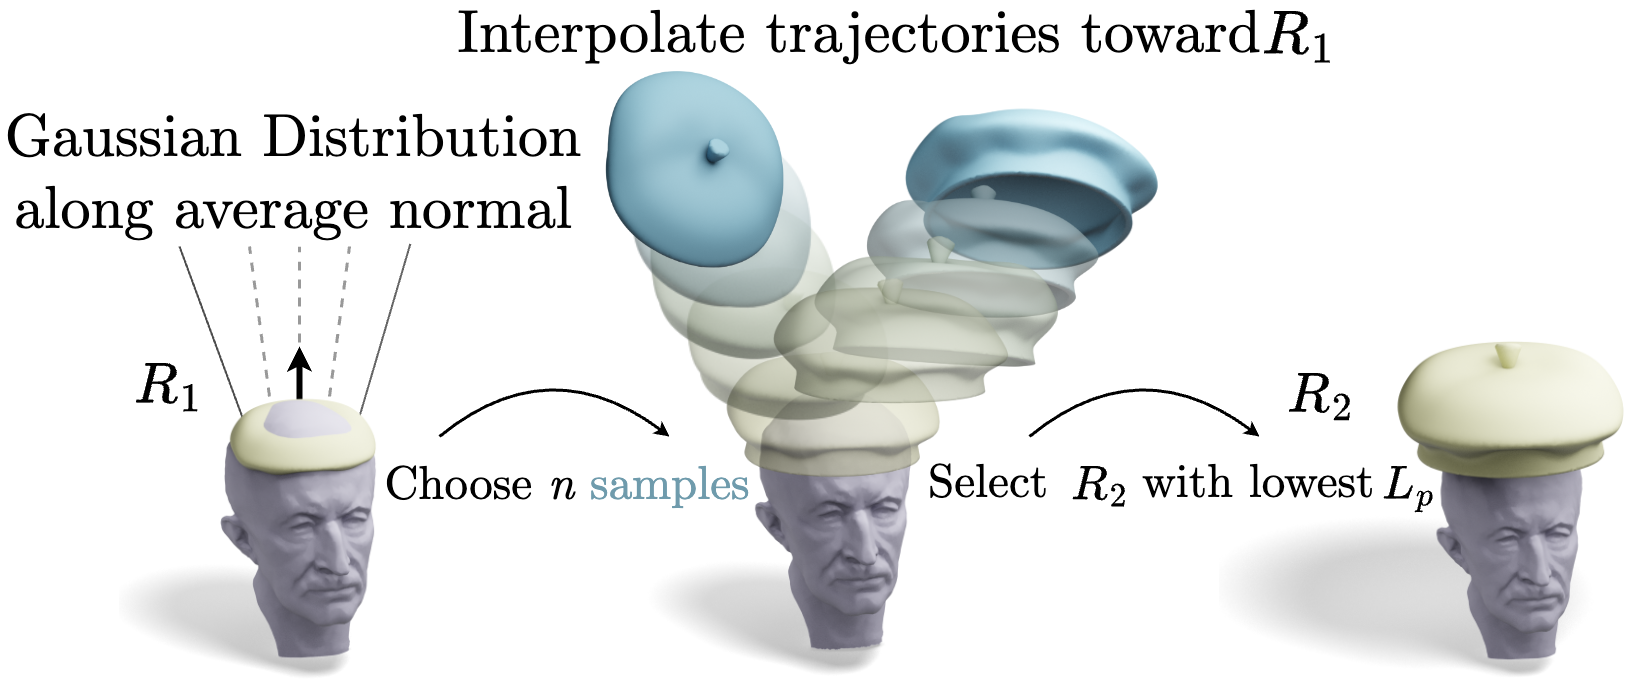
\includegraphics[width=\linewidth]{figures/trajectory_method/trajectory_method.png}
    \caption{}
    % \caption{To find a non-intersecting configuration, we simulate several possible object trajectories and sample different timesteps (see \autoref{sec:step2}). Among all non-intersecting candidates, we select the one closest to the target region of the base mesh.}
    \label{fig:trajectory_method}
\end{wrapfigure}

Once $\rigid^1,\dots,\rigid^{\numnonintersecting}$ have been identified, we use spherical linear interpolation (SLERP) to build candidate trajectories from each non-intersecting $\rigid^i$ to the intersecting transformation from the previous step $\rigid_1$ (see \autoref{fig:trajectory_method}, transparent frames). We sample $\numtimesteps$ discrete timesteps of each trajectory, keeping only the non-intersecting ones (in our experiments, $m=25$). After gathering all non-intersecting timesteps for all candidate trajectories $R^i$, we make $\rigid_2$ be the transformation with the lowest proximity loss $\mathcal{L}_{p}$ (\autoref{fig:trajectory_method}, right).

\begin{figure*}[t]
    \centering
    \vspace{3mm}
    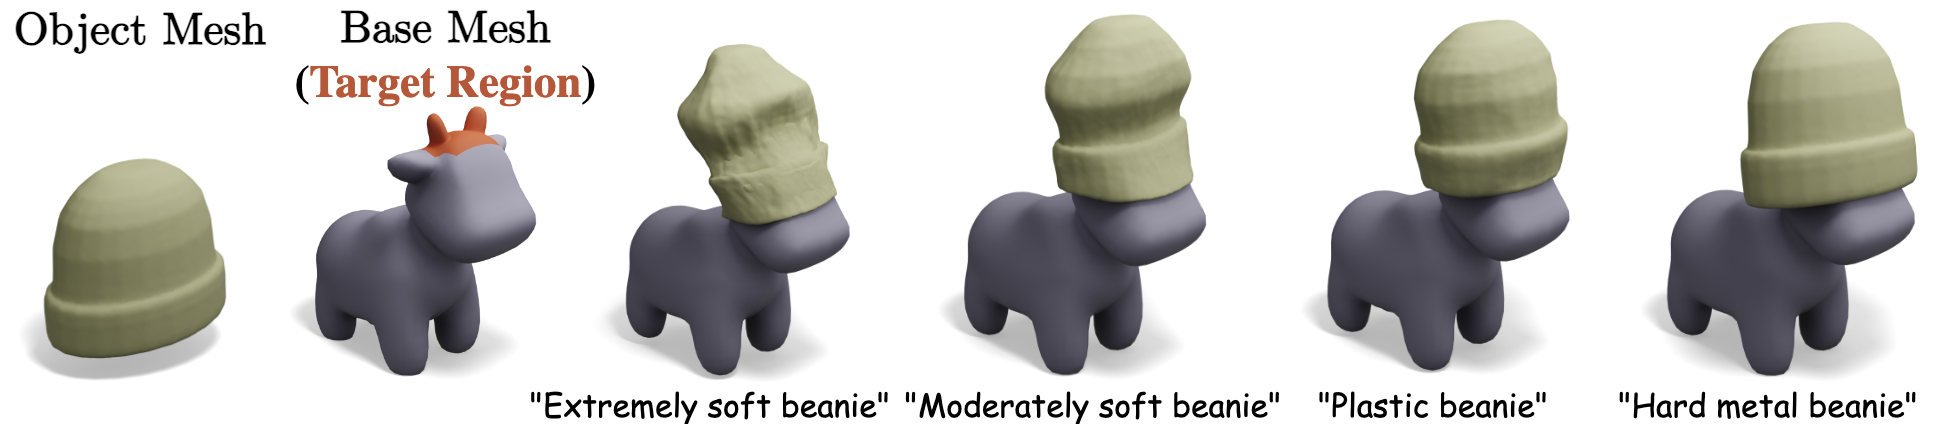
\includegraphics[width=\textwidth]{figures/materials/materials.png}
    \captionof{figure}{\ourmethod{} is capable of fitting the accessory onto the base mesh in a way that considers material properties. Instead of having to specify the numeric material parameters, artists can provide material guidance through text prompts, that get combined with rendered images and interpreted by a VLM to output specific elastic parameters.}
    %\vspace{-2cm}
    \label{fig:materials}
\end{figure*}%





\subsection{Step 3: Rigid finetuning}
\label{sec:step3}
The output of the previous section is a (scaled) rigid transformation $\rigid_2$ that moves the accessory reasonably close to the highlighted region of the base mesh without intersecting it; however, it likely fits too loosely to seem realistic (see \autoref{fig:main_method}, middle).

To refine this transformation, we draw inspiration from works in the physically-based simulation area, in which the relative positions of many objects are often assumed to minimize some physically meaningful energy (e.g., gravity) subject to non-intersecting constraints.
A common strategy for imposing these constraints is by adding repulsive energy terms to the optimization \cite{baraff1998large,li2020incremental,lan2024efficient}.
In a similar way, starting from $\rigid_2 = \rigid(\parameters_2)$, we will optimize the loss
\begin{equation}\label{equ:total-loss}
\mathcal{L}(\parameters) = \mathcal{L}_{p}(\parameters) + \mathcal{L}_{\text{IPC}}(\parameters)\,,
\end{equation}
where $\mathcal{L}_{p}$ is the proximity loss introduced in \autoref{sec:step1} and $\mathcal{L}_{\text{IPC}}$ is the \emph{Incremental Potential Contact} barrier energy \cite{li2020incremental}, given by
\begin{equation*}
\mathcal{L}_{\text{IPC}}(\parameters) = \sum_{\vertex_i \in \objectmesh} b_{\contactthreshold}\left(d\left(\rigid(\parameters)\vertex_i,\basemesh\right)\right)\,,
\label{contact_loss}
\end{equation*}
where
\begin{equation*}
    b_h(x) =
    \begin{cases}
      -(x-h)^{2}\ln\left( \dfrac{x}{h} \right) & \text{if}\quad x < h \\
      0       & \text{otherwise.}
    \end{cases}
\end{equation*}
This energy penalizes the object's vertices as they approach the base surface, with a second-order continuous (\( C^2 \)) form at the boundary \( d\left(\rigid(\parameters)\vertex_i,\basemesh\right) = \contactthreshold \), and naturally vanishes as \( d\left(\rigid(\parameters)\vertex_i,\basemesh\right) \to \contactthreshold \) or beyond (in our experiments, $h=0.01$). In addition to its use as an optimization energy in this section, we also use $\mathcal{L}_{\text{IPC}}$ to classify if a configuration is or not intersecting in the previous sections.

Minimizing the total loss from \autoref{equ:total-loss} using gradient-based optimization, starting from $\rigid_2$, results in a novel (scaled) rigid transformation $\rigid_3 = \rigid(\parameters^\star)$ that fits the object tightly without intersections over the base mesh.



\begin{figure*}[t]
\vspace{3mm}
\centering
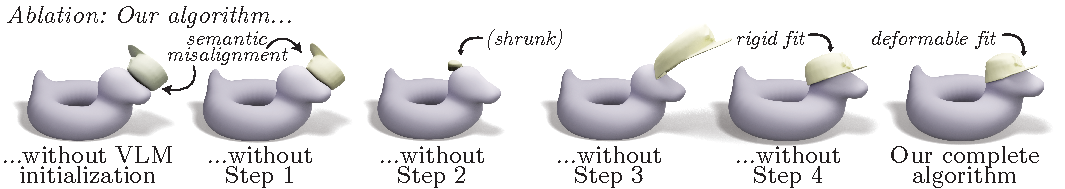
\includegraphics[width=\textwidth]{figures/placeholders/steps-ablation.pdf}
\caption{\ourmethod{} uses a multi-step process, where each of them is critical for achieving a desirable mesh to mesh composition result. Omitting any of the steps yields a semantically (two left results) or physically (two center results) unplausible solutions. Utilizing Step 4 further improves the result (second from the right), allowing the asset to deform and better fit the base mesh (rightmost).} %\rana{something more about what }
\label{fig:steps-ablation}
\end{figure*}



\subsection{Step 4: Elastic deformation}
\label{sec:step4}

The physically-inspired optimization of the previous step outputs a rigidly transformed mesh $\restmesh = \rigid_3 (\objectmesh) = ( \rigid_3 (\objectverts), \objectfaces)$, which we interpret as the best possible \emph{rigid fit} of the object onto the base mesh.
In reality, however, many accessories fit their wearer more tightly by undergoing small deformations: a hat is stretched by a head's shape, a necklace drapes over a person's chest, a face mask deforms to fit the nose and mouth of a surgeon.
Beyond physical deformation, an artist may also wish to perform small physical non-rigid edits on a general-purpose object mesh to better match their specific creative intentions.

To model this final fit, we will follow the lead of prior work \cite{aigerman2022neural, kim2025meshup, gao2023textdeformer, dinh2025geometry} and parametrize the object mesh deformation via a per-face Jacobian field \( \{J_i \in \mathbb{R}^{3 \times 3}\} \), which describes the local transformation of the surface. From these Jacobians, one can recover vertex-wise deformations $ \vertext_i = \transformation (\vertex_i) $  through a Poisson-like least-squares minimization:
\begin{equation}\label{equ:poisson}
\transformation^\star = \arg\min_t \sum_i a_i \left\| \nabla_i(t) - J_i \right\|_2^2\, ,
\end{equation}
where $a_i$ is the area of the $i$-th triangle in the mesh. This allows us to write $\transformation$ as a function of the per-face Jacobians $\transformation = \transformation(J_1, J_2, \dots) = \transformation(\{J_i\})$.
Our proximity and IPC losses from the previous section can thus be analogously defined for this non-rigid setting as
\begin{align}
\mathcal{L}_{p}(\{J_i\}) & = \sum_{\vertex_{i} \in \objectmesh} \hat{d} (\transformation(\{J_i\})\vertex_i, \highlightedmesh)^2  
+  \sum_{\vertex_{j} \in \highlightedmesh} \hat{d}(\vertex_j, \transformation(\{J_i\})\objectmesh)^2\,
\end{align}
and
\begin{align}
\mathcal{L}_{\text{IPC}}(\{J_i\}) & = \sum_{\vertex_i \in \objectmesh} b_{\contactthreshold}\left(d\left(\transformation(\{J_i\})\vertex_i,\basemesh\right)\right)\,,
\end{align}
where we use a lower proximity threshold value of $\ell=0.01$ to zero out distance entries, enforcing the deformation to be conservatively confined to its local boundries. 
The point-to-mesh distances $d$ are once again computed using a bounding volume hierarchy; however, this hierarchy is recomputed every $20$ iterations due to the presence of deformations.
Additionally, we follow the strategy proposed by \emph{MeshUp} \cite{kim2025meshup} and guide the deformation towards a semantically meaningful fit via Score Distillation Sampling (SDS).
Let \( z \) denote a rendered image of the current mesh, and \( \mathcal{T} \) a guiding text prompt. At each iteration, we sample a timestep \( t \sim \mathcal{U}(0,1) \) and a noise vector \( \epsilon \sim \mathcal{N}(0,I) \), and use the gradient
$$
\nabla_{J_i} \mathcal{L}_{\text{SDS}}(\{J_i\}) = w(t)\left(
\epsilon_\omega(z_t, \transformation(\{J_i\}), t) - \epsilon
\right)
\cdot
\frac{\partial z_t}{\partial J_i}.
$$
Finally, some deformations are more physically realistic than others, and different materials will deform by different amounts. To model this, we include the standard elastic NeoHookean energy as a loss term (see \cite{sifakis2012fem}, Chap. 3.6),
\begin{align*}
\mathcal{L}_e (\{J_i\}) = & \sum_i \left(\frac{\mu}{2}\left(\tr(J_i^\top J_i) - 3\right)\right.
- \left.\mu \log(\det(J_i))
 + \frac{\lambda}{2} \log^2(\det(J_i)) \right)
\end{align*}
where the material parameters $\lambda$ and $\mu$ are either given as input to our algorithm or inferred either from rendered images or text descriptions by our multi-agent initialization framework (see \autoref{sec:initialization}).
We end by minimizing the total loss
\[
\mathcal{L} = \mathcal{L}_{p} + \mathcal{L}_{\text{IPC}} + \lambda_{\text{SDS}} \mathcal{L}_{\text{SDS}} + \lambda_{e} \mathcal{L}_e\, ,
\]
with respect to $\{J_i\}$ using gradient-based optimization, and solve \autoref{equ:poisson} to obtain our final transformation $\transformation$ (see \autoref{fig:main_method}, right). As desired, $\transformation$ fits the object mesh tightly onto the base mesh in a semantically and physically realistic way without intersections, ending our algorithm.





\subsection{Initialization}
\label{sec:initialization}
Like any gradient-based optimization, our algorithm is sensitive to initialization; in particular, it depends on the initial relative configuration of the two meshes that is then modified in steps one through four.
Experimentally, we find that our method is relatively robust to different initial configurations; however, the most adversarial of them can cause it to converge to undesirable local minima (see \autoref{fig:initialization}).

To avoid these, we initialize the relative configuration using a VLM.  First, from a text description (e.g., "a hat") and renderings of the object, the VLM is prompted to produce a canonical reference frame for it (e.g., "the front of the hat is the region with a visor, the top part of the hat...."). This process is repeated for the base mesh. Then, several different random orientations are sampled for the object mesh. For each, a VLM is used to deduce its alignment with the canonical reference frame and with the base mesh's. The latter is used to score each configuration, and we select the highest-scoring one as initialization (see Supplementary Material for details). 


 An additional agent uses user input text to output the the material parameters $\lambda, \mu$, giving users a fully-integrated, text-based control over the entire optimization process (see \autoref{fig:main_method}).
More details about our initialization scheme are provided in the Supplementary.

\section{Experiments} \label{sec:experiments}





Our algorithm is implemented in Python using \textsc{PyTorch} for autodifferentiation. Our comparisons to Iterative Closest Point and its derivative works, Deep Closest Point \cite{wang2019deep}, and Instant3dit \cite{barda2025instant3dit} use official or publicly available implementations \cite{Zhou2018}. We render our results using \textsc{Blender}, and provide more implementation details in the Supplementary Materials.

% bvh
As is theoretically expected, our main computational bottleneck is the calculation of point-to-mesh distances involved in the proximity and IPC losses $\mathcal{L}_p$ and $\mathcal{L}_{IPC}$.
Our tailor-made BVH reduces the computational cost of this step, allowing us to produce results for relatively large meshes within reasonable times (see Supplementary).


\begin{wrapfigure}[10]{r}{0.50\linewidth}
    \vspace{-4mm}
    \centering
    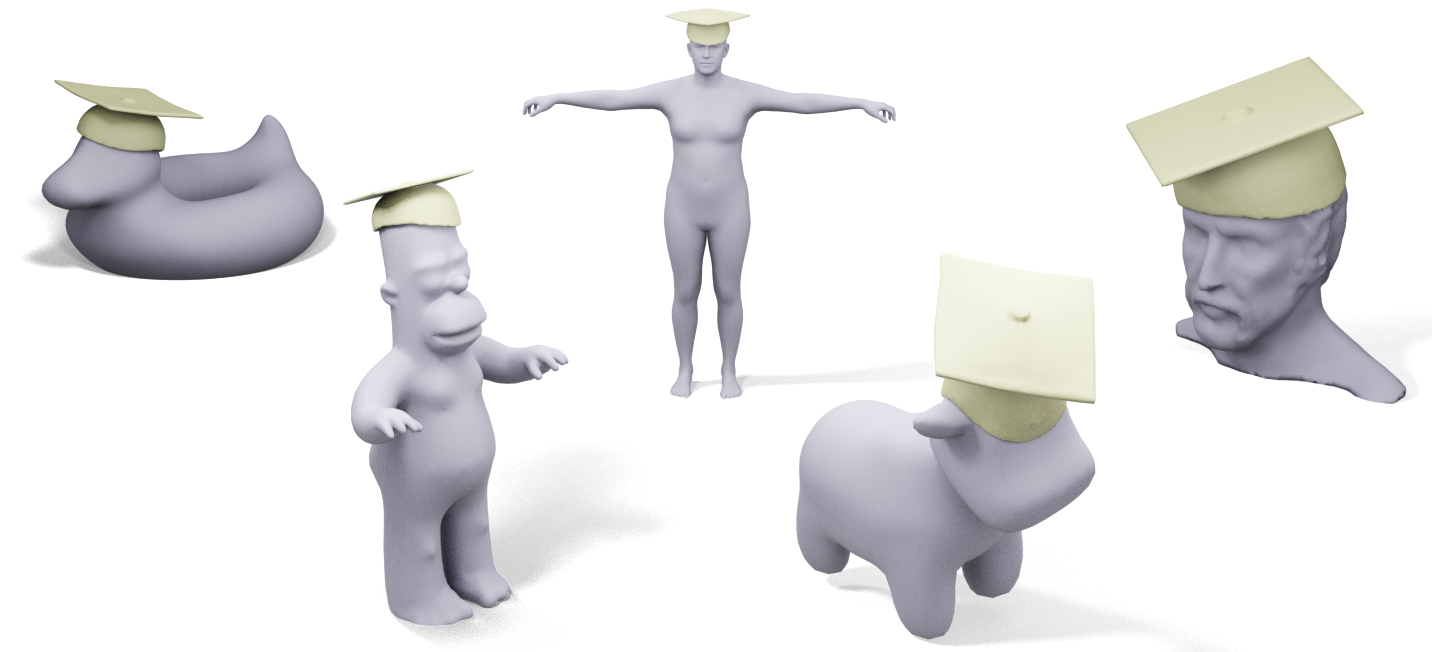
\includegraphics[width=\linewidth]{figures/same_accesory_different_base/same_accesory_different_base.png}
    \caption{}
    % \caption{Our method fits the same accessory on different base meshes, adapting to differences in scale, head shape, and body proportions to place the asset in a semantically correct position.}
    \label{fig:same_accesory_different_base}
\end{wrapfigure}





\begin{figure*}[t]
    \vspace{3mm}
    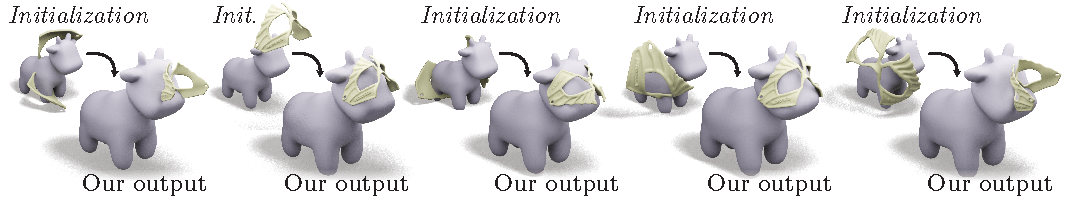
\includegraphics[width=\textwidth]{figures/placeholders/initialization.pdf}   
    \caption{Our method is moderately robust to different initialization configurations, although it can fail to converge to the desired output in very adversarial cases (leftmost and rightmost). In \autoref{sec:initialization}, we introduce a VLM initialization strategy that avoids these cases.}
    \label{fig:initialization}
    \vspace{-4mm}
\end{figure*}


% highlight robustness
A particularly relevant set of parameters are the material elastic properties $\lambda$ and $\mu$, which can be derived from the material's Young's modulus and Poisson's ratio \cite{sifakis2012fem}.
These quantities are tabulated for well-known materials; however, we make the process more intuitive for an artist by assigning the values from text inputs using an LLM. We explore both the VLM assignment and the effect of these parameters in \autoref{fig:materials}, in which the object is allowed to deform more or less depending on the specified material.

As expected, our algorithm's output is most sensitive to the selected target region on the base mesh $\highlightedfaces\subset \basefaces$.
In \autoref{fig:highlight-region}, we show how this input can allow artists to select different semantically meaningful assembly configurations between the two objects in ambiguous cases.
A similar example is given in \autoref{fig:four_fingers}, where different highlight regions specify the finger wearing a ring.



To obtain a tight, non-intersecting fit between the base and the accessory, our algorithm relies on a VLM-driven initialization and four successive optimizations, the input and output of each we show in \autoref{fig:main_method}. In \autoref{fig:steps-ablation}, we show the importance of each of these steps: skipping the VLM initialization results in a non-semantic fit (a backwards hat), while skipping any of the intermediate steps results in outputs with significantly worse physical and geometric fit. As expected, skipping Step 4 results in a strictly rigid fit, while enabling Step 4 allows the object to deform.

Critically, in Step 2 of our algorithm (\autoref{sec:step2}), we sample trajectories to find a close, non-intersecting configuration. We exemplify this in \autoref{fig:trajectory_method}; as shown in \autoref{fig:steps-ablation}, skipping this causes the barrier term in Step 3 to greatly displace the shape away from the base mesh.



\section{Comparisons} \label{sec:comparisons}
% ICP and deep closest point
\subsection{Qualitative Evaluation}
Inspired by the digital artists' workflows, we consider the specific question of how to align two pre-existing shapes in a semantically meaningful, non-intersecting, tight way.
While the lack of prior work dedicated to this particular problem makes direct comparisons difficult, we justify the need for our method by showing the failure of existing general-purpose algorithms when applied to this task.

For example, by finding an alignment between two 3D objects, our method can be seen as a special kind of \emph{registration} algorithm. However, unlike standard registration algorithms, we do not rely on the existence of a rigid geometric match between the two objects: as shown in \autoref{fig:materials}, the accessory may need to deform significantly for it to even be a partial match of the base mesh.

\begin{figure}[t]
    \vspace{3mm}
    \centering
    
    \begin{subfigure}[t]{0.49\linewidth}
        \centering
        \begin{minipage}[t][0.8cm][t]{\linewidth}
            \centering\textbf{(a) Ring Placement}
        \end{minipage}
        \phantomsubcaption\label{fig:four_fingers}
        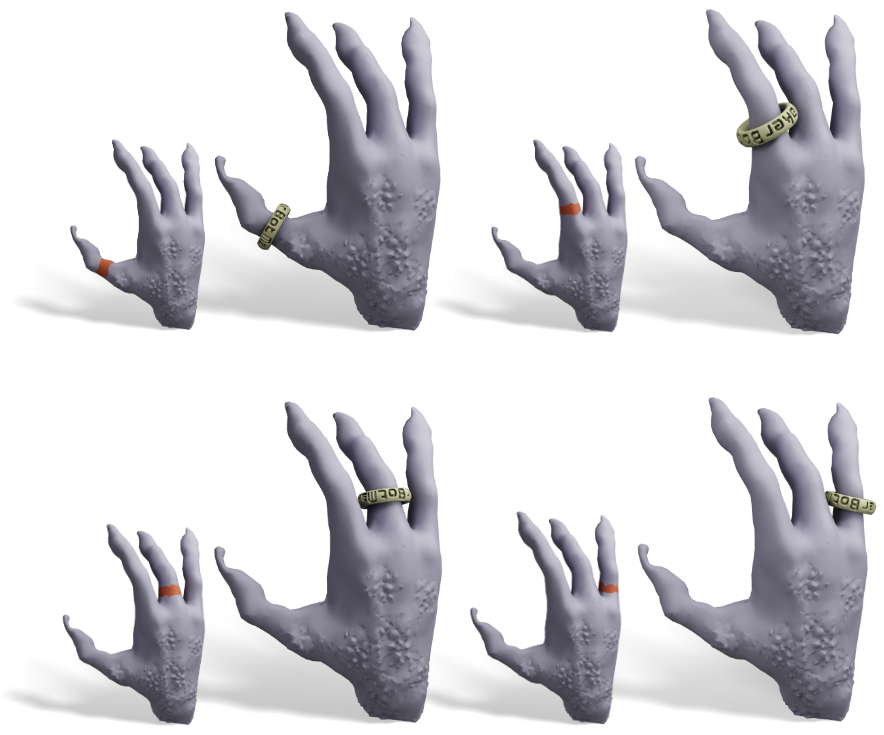
\includegraphics[width=\linewidth]{figures/region_control/four_fingers.png}
    \end{subfigure}
    \hfill
    \begin{subfigure}[t]{0.49\linewidth}
        \centering
        \begin{minipage}[t][0.8cm][t]{\linewidth}
            \centering\textbf{(b) Region Sensitivity}
        \end{minipage}
        \phantomsubcaption\label{fig:highlight-region}
        
\includegraphics[width=\linewidth]{figures/region_control/highlight-region-2-2.pdf}
    \end{subfigure}

    \vspace{3mm}
    \caption{
    \textbf{Region-controlled composition.}
    \textbf{(a)} Given four distinct user-selected target regions, \ourmethod{} places a ring precisely on each selected region, demonstrating explicit user control over the fitting process.
    \textbf{(b)} Because the method adheres strictly to the selected region, asset placement is sensitive to the region definition; for example, glasses sit naturally on the ears only if a small portion of the ear region is included in the selection.
    }
    \label{fig:region_control}
\end{figure}

More importantly, general shape registration algorithms, which are often used with point cloud inputs, will cause significant intersections between the base mesh and the object.
We show examples of this phenomenon in \autoref{fig:comparison}, where we compare our method to variants of classical registration methods \cite{besl1992method}\footnote{\label{fn:alignment_baseline}Classical registration methods are highly sensitive to bad initialization, so we use their variants that are known to be more robust. More details can be found in the Supplementary Materials.}.
Additionally, non-neural methods like those based on the Iterative Closest Point algorithm will not account for the semantic fit between the two objects; \eg, fitting the glasses backwards on the face.
We also experimented with public implementations of data-driven methods like Deep Closest Point \cite{wang2019dcp}; however, we found that these struggle greatly with most standard shapes outside of their training data, when restricted to the highlighted target region.

By modifying a shape using diffusion guidance, a highlighted region, and an optional text prompt, our work may seem similar to existing text-guided generative mesh-editing works.
Unlike these, however, our work preserves both the object and base meshes as well as any information stored in them.
Taking Instant3dit \cite{barda2025instant3dit} as a representative example, we show the difference between ours and this class of methods in \autoref{fig:instant3dit_comparison}.
Instant3dit produces a generative edit that merges the geometry of both objects and discards the animation rig of the base mesh and the parametrization of the accessory.
By contrast, our method places a world of possibilities in the hands of the artist by preserving all these, enabling common downstream tasks like animation, physical simulation, and texture painting.

\begin{figure*}[t]   
    \vspace{3mm}
    \centering
    % \vspace{-0.5cm}
    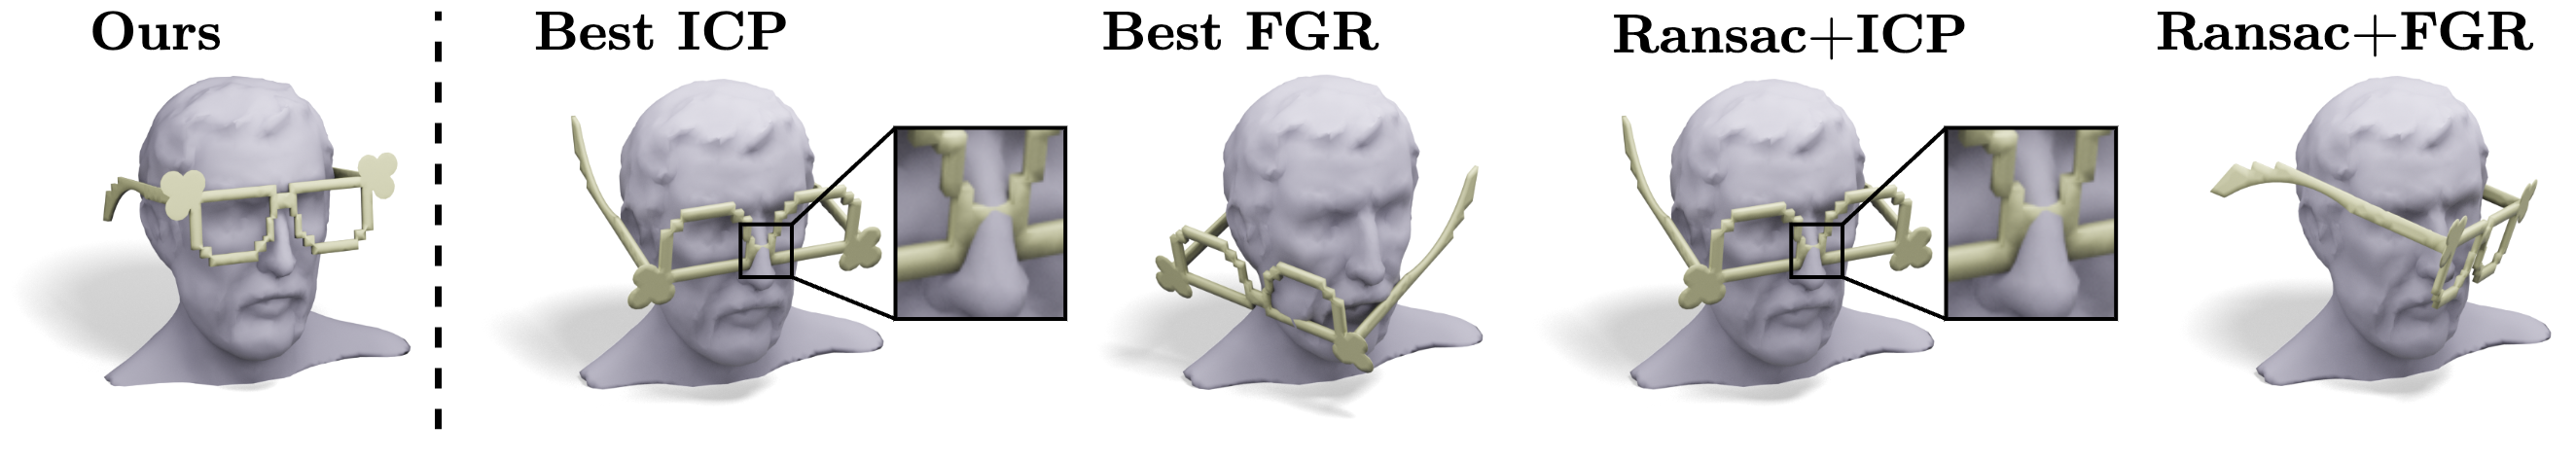
\includegraphics[width=\textwidth]{figures/comparison/comparison.png}
        \captionof{figure}{Unlike ours (left), classical registration algorithms like ICP contain no semantic guidance: therefore, they will produce unrealistic configurations; e.g., glasses that sit on the eyes upside down. These algorithms are also not designed to avoid intersections; therefore, they will produce many of them (see blowups). See supplementary materials for details of these methods.}
    %\vspace{-2cm}
    \label{fig:comparison}
\end{figure*}%



\subsection{Quantitative Evaluation.}
We quantitatively evaluate our method along two complementary dimensions: semantic alignment quality and geometric validity. We also show a user study of semantic alignment in the Supplementary Materials.\\

In \autoref{tab:quant_all}, we  compare our method against multiple alignment baselines, including Instant3Dit~\cite{barda2025instant3dit}, Best ICP/FGR, and RANSAC-based variants~\ref{fn:alignment_baseline}.  
We measure semantic quality using VQA~\cite{lin2024evaluating} and two CLIP-based metrics~\cite{radford2021learning,wang2023exploring} on image renderings of ten examples. We post examples of these renderings in the Supplementary Materials.
Across these metrics, our full method achieves the strongest or near-strongest performance (for CLIP-IQA scores, the margin is $0.006\text{--}0.009$).
Alignment-based methods also frequently produce mesh intersections, an undesirable artifact for most graphics workflows. 
In \autoref{tab:penetration} we report total intersecting faces and maximum penetration depth for each for these methods, demonstrating that while all baseline methods exhibit substantial intersections, our method produces intersection-free compositions. 







\section{Applications} \label{sec:applications}
% teaser
% same accessory, different base mesh
% gallery
% different regions, same meshes
% beanie
Since our method is designed to fit directly into artists' workflows, we prioritize providing them with the highest degree of control over the fit, automating only the tedious rigid and deformable fitting procedure.
With our method, artists may specify every creative detail: from the input meshes and their properties, which are preserved (see \autoref{fig:instant3dit_comparison}), to the accessory's material parameters (see \autoref{fig:materials}) and the specific region of the fit (see \autoref{fig:four_fingers}).

\begin{table}[t]
\vspace{4mm}
\centering
\small
\setlength{\tabcolsep}{6pt}
\renewcommand{\arraystretch}{1.2}
\setlength{\aboverulesep}{0pt}
\setlength{\belowrulesep}{0pt}

\resizebox{\columnwidth}{!}{%
\begin{tabular}{lcccccc}
\toprule
\multicolumn{7}{l}{\textbf{Alignment Baselines}}\\
\rowcolor{headercolor}
Metric & \shortstack{Instant3Dit} & \shortstack{Best ICP} & \shortstack{Best FGR} & \shortstack{RANSAC+ICP} & \shortstack{RANSAC+FGR} & \shortstack{Ours} \\
\midrule
\rowcolor{zebra}
CLIP ($\uparrow$)     & 0.311 & 0.341 & 0.333 & 0.331 & 0.321 & \textbf{0.356} \\
CLIP-IQA ($\uparrow$) & 0.559 & 0.586 & 0.609 & 0.608 & \textbf{0.610} & 0.604 \\
\rowcolor{zebra}
VQA ($\uparrow$)      & 65.62 & 73.71 & 73.97 & 73.72 & 73.68 & \textbf{74.49} \\
\midrule
\\[4pt] 
\midrule
\multicolumn{7}{l}{\textbf{Ablation Study}}\\
\rowcolor{headercolor}
Metric & \shortstack{Init} & \shortstack{Step 1} & \shortstack{Step 2} & \shortstack{Step 3} & \shortstack{Step 4} & \shortstack{Ours} \\
\midrule
\rowcolor{zebra}
CLIP ($\uparrow$)     & 0.338 & 0.351 & 0.346 & 0.347 & 0.354 & \textbf{0.356} \\
CLIP-IQA ($\uparrow$) & 0.594 & 0.605 & 0.609 & 0.595 & \textbf{0.613} & 0.604 \\
\rowcolor{zebra}
VQA ($\uparrow$)      & 74.197 & 73.967 & 73.776 & 74.049 & 73.985 & \textbf{74.49} \\
\bottomrule
\end{tabular}%
}
\vspace{4mm}
\caption{Quantitative evaluation using CLIP, CLIP-IQA, and VQA scores. Top: comparison against alignment baselines. Bottom: ablation study of our multi-step pipeline. Scores are averaged over per-example best renderings (best of 4); higher is better.}
\vspace{-2mm}
\label{tab:quant_all}
\end{table}

We exemplify our algorithm's applicability through several prototypical examples. As shown in \autoref{fig:gallery}, our method can find tight, non-intersecting configurations between a diverse range of meshes, even when these contain complex geometries, concavities, and topologies.
In \autoref{fig:teaser}, successive pre-existing shapes are added to an existing model to create a superhero character.
Conversely, in \autoref{fig:same_accesory_different_base}, the same accessory is automatically placed on a wide range of characters, demonstrating how our method can adapt to different scales, head shapes, and body proportions.



\begin{table}[t]
\vspace{4mm}
\centering
\small
\setlength{\tabcolsep}{3pt}
\renewcommand{\arraystretch}{1.15}

\begin{tabularx}{\linewidth}{>{\raggedright\arraybackslash}X c c c c c}
\toprule
{\textbf{Ablation Study}}\\
\rowcolor{headercolor}
Metric &
Best ICP &
Best FGR &
RANSAC+ICP &
RANSAC+FGR &
Ours \\
\midrule
\rowcolor{zebra}
Intersecting faces ($\downarrow$)
& 628 & 660 & 544 & 434 & \textbf{0} \\
Max penetration ($\downarrow$)
& 0.0197 & 0.0237 & 0.0243 & 0.0237 & \textbf{0} \\
\bottomrule
\end{tabularx}
\vspace{4mm}
\caption{Penetration statistics averaged over ten experiments. We report the total number of intersecting faces and the maximum penetration depth. Our method produces intersection-free compositions (all zeros).}
\vspace{-3mm}
\label{tab:penetration}
\end{table}




  
\section{Conclusion} \label{sec:conclusion}
We introduced a mesh composition algorithm that produces a meaningful, tight, non-intersecting fit between two shapes, inspired by the application of 3D digital art.
For our work to be useful in an interactive, real-time 3D modeling session, however, its runtime would need to improve significantly.
We believe there are several potential avenues for this: for example, one could dramatically improve runtimes by building increasingly fine nested simulation cages using existing methods \cite{sacht2015nested}. Then, one could perform the optimizations in our algorithm successively for each refinement level, thus reducing the need for extensive computation on the finest of levels.

As a tool of artist control, our algorithm requires a user to specify a highlighted region of the base object onto which the accessory should be attached. Experimentally, we find that our algorithm's output is sensitive to small changes in this region (see \autoref{fig:highlight-region}), which could lead to user frustration.
This issue could be resolved by future work combining our algorithm with existing text-based mesh selection tools like \emph{3D Highlighter} \cite{decatur20233d}.




As a final step in our fit, our algorithm allows the object to deform in order to better match the base mesh.
This results in an improved fit (see \autoref{fig:steps-ablation}) and provides an additional avenue for artist control (see \autoref{fig:materials}).
However, our method still assumes mostly-rigid scenarios in which the attachment to the base mesh is the main source of deformation.
For fundamentally elastic materials in which other internal and external forces are dominant (\eg, a piece of cloth draping over a character), a better fit can likely be achieved with existing physical simulation tools.

This is a time of friction between rapidly improving 3D AI research and artist communities reluctant to incorporate these tools due to loss of control and creativity.
While solving this friction is a complex problem beyond the scope of any one paper, we hope that non-generative AI-driven tools like \ourmethod{}, which is intended to fit directly into real digital artists' workflows while maximizing creative control, can aid in building bridges between these two worlds.
%\input{06_acknowledgements.tex}
\input{07_figures_only_pages.tex}
{
    \small
    \bibliographystyle{ieeenat_fullname}
    \bibliography{references}
}

% WARNING: do not forget to delete the supplementary pages from your submission 
% \input{sec/X_suppl}

\end{document}
